\section{TUTORIAL: Imágenes}
\subsection{Imagen centrada}
En esta plantilla hay 2 formas de incluir imágenes. La primera es la más compleja y manual que aparece en el código comentado.
%\begin{figure}[H] % IMPORTANTE en la mayoria de los casos, alternativas: [h],[t],[b],[p],
%    \centering
%    \begin{measuredfigure} % Lo usamos para aliniar el caption
%        \caption{Título de la imagen} % IMPORTANTE que este arriba
%        
\includegraphics[width=0.2\textwidth]{img/cuadradoejemplo.png} % Alternativa \includegraphics[height=3cm]{}
%        \label{img:referencia0}
%    \end{measuredfigure}
%\end{figure}

La segunda forma de incluir imágenes es la más sencilla, solo se tiene que usar el comando personalizado:
\begin{verbatim}
\fig[label]{Titulo}{tamaño}{ruta_imagen}
Ejemplo:
\fig[referencia1]{Titulo de la imagen 1}{width = 0.2\textwidth}{img/cuadradoejemplo.png}
\end{verbatim}

\fig[referencia1]{Titulo de la imagen 1}{width = 0.2\textwidth}{img/cuadradoejemplo.png}

% Tambien se puede agregar sin caption ni label ni titulo:
% \fig{}{width = 0.2\textwidth}{img/cuadradoejemplo.png}

\subsection{Imágenes alineadas}
Si se desea incluir una imagen a la izquierda o derecha de un párrafo, se puede consultar nuevamente el codigo comentado o usar el siguiente comando (Poniendo \{r\} o \{l\} dependiendo del caso):
\begin{verbatim}
\figposition[label]{Titulo}{tamaño}{ruta_imagen}{posicion_r/l}
Ejemplo:
\figposition[referencia2]{Imagen referencia }{height=3cm}{img/cuadradoejemplo.png}{r}
\end{verbatim}

\figposition[referencia2]{Imagen referencia }{height=3cm}{img/cuadradoejemplo.png}{r}

% FORMA MANUAL:
%\begin{wrapfigure}{r}{0.25\textwidth} % Margen del texto
%    \centering
%    \begin{measuredfigure}
%        \caption{Imagen referencia 2}
%        
\includegraphics[height=3cm]{img/cuadradoejemplo.png} %[scale=0.1]
%        \label{img:referencia2}
%    \end{measuredfigure}
%\end{wrapfigure}


\textcolor{silver}{
    Lorem Ipsum is simply dummy text of the printing and typesetting industry. Lorem Ipsum has been the industry's standard dummy text ever since the 1500s, when an unknown printer took a galley of type and scrambled it to make a type specimen book. It has survived not only five centuries, but also the leap into electronic typesetting, remaining essentially unchanged.
    }

\newpage

%%%%%%%%%%%%%%%%%%%%%%%%%%%%%%%%%%%%%%%%%%%%%%%%%%%%%%%
\section{TUTORIAL: Tablas}

Hacer tablas en \LaTeX es muy engorroso, por lo que presentamos 3 alternativas. Sin embargo, es necesario aclarar que para que se respete el formato de las tablas, \textbf{se tiene que poner el catión SOBRE la tabla.}

\subsection{Generador online}
Hay muchas páginas para generar tablas automáticamente, una alternativa es \href{https://www.tablesgenerator.com}{tablesgenerator}, sin embargo, este método genera muchas líneas innecesarias y cuando se incorporan párrafos muy grandes hay que ajustar las palabras.

\subsection{Insertar una imagen como tabla}
Se puede incorporar una imagen (De Excel, por ejemplo) como si fuera una tabla. El único inconveniente es que no va a permitir seleccionar el texto en el pdf generado. Al igual que con las imágenes, hay un comando personalizado y un código manual comentado.\footnote{\textit{Si no se quiere incluir el texto opcional, pueden dejar vacío la última celda (\{\})}}
\begin{verbatim}
\tableimage[label]{Titulo}{tamaño}{ruta_imagen}{Texto_referencia}
Ejemplo:
\tableimage[referencia3]{Tabla de referencia 1}{height=3cm}{img/tablaejemplo.png}{Texto}
\end{verbatim}



\tableimage[referencia3]{Titulo de la tabla de referencia}{height=3cm}{img/tablaejemplo.png}{Fuente de los datos}

% Tabla manual:
%\begin{table}[H]
%    \centering
%    \begin{measuredfigure}
%        \caption{Tabla de referencia 1}
%        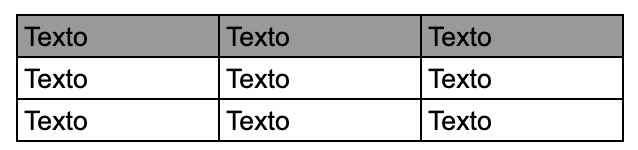
\includegraphics[height=3cm]{img/tablaejemplo.png}
%        \label{img:referencia3}
%    \end{measuredfigure}
%    \\ \textit{\scriptsize{Texto opcional al el pie de Tabla.}}
%\end{table}

\newpage
\subsection{Usar plantilas}
Pueden copiar y modificar el codigo siguiente:

\begin{minipage}[H]{0.49\textwidth}
    \begin{table}[H]
        \centering
        \begin{measuredfigure}
            \caption{Tabla de referencia 2}
            \begin{tabular}{| l | c | r |}
            \hline
                \textbf{Texto} & \textbf{Texto} & \textbf{Texto} \\ \hline
                Textoblabla    & Textoblabla   & Textoblabla \\ \hline
                Texto    & Texto   & Texto \\ \hline
            \end{tabular}
        \end{measuredfigure}
        \\ \textit{\scriptsize{Fuente de los datos.}}
    \end{table}
\end{minipage}
\begin{minipage}[H]{0.49\textwidth}
    \begin{table}[H]
        \centering
        \begin{measuredfigure}
            \caption{Tabla de referencia 3}
            \begin{tabular}{l l l}
            \toprule
                \textbf{Texto} & \textbf{Texto} & \textbf{Texto} \\
                \midrule
                Textoblabla    & Textoblabla   & Textoblabla \\
                Texto    & Texto   & Texto \\
                \bottomrule
            \end{tabular}
        \end{measuredfigure}
        \\ \textit{\scriptsize{Fuente de los datos.}}
    \end{table}
\end{minipage}
\newpage

%%%%%%%%%%%%%%%%%%%%%%%%%%%%%%%%%%%%%%%%%%%%%%%%%%%%%%%
\section{TUTORIAL: Citación}

Para citación extensa en formato APA, citas con más de 40 palabras, se sugiere el uso del siguiente comando personalizado:

\begin{verbatim}
    \quotex{cita}
    Ejemplo:
    \quotex{\lipsum (Autor, Año)}
\end{verbatim}

\quotex{\lipsum (Autor, Año)}

Puedes realizarlo de forma manual modificando el código comentado

%Cita extensa APA manual:

%\begin{flushright}
%    \begin{minipage}{0.96\linewidth}
%        \vspace{5pt}
%        {\small
%            %Acá va la cita
%        }
%        \vspace{5pt}
%    \end{minipage}
%\end{flushright}
